%SourceDoc ../YourName-Dissertation.tex
%\vspace*{-80mm}
\chapter{Introduction} \label{chapter1:introduction}

\section{Motivation}
Al$_{2}$O$_{3}$ is arguably the most extensively used and resarched ceramic material with a total estimated market of 2.8 million tons per year.  The applications for Al$_{2}$O$_{3}$ vary drastically such as high temperature refractories, technical ceramics, high voltage insulators, and functional fillers. Bayer feedstocks make a majority of the syntetic and specialty aluminas used in Al$_{2}$O$_{3}$ applications, such as aluminum trihydrate (Al(OH)$_{3}$), smelter grade Al$_{2}$O$_{3}$ and others. Bayer process aluminas typically have a purity between 99.0 - 99.9\% and contain impurities such as, Na$_{2}$O, CaO, Fe$_{2}$O$_{3}$, and SiO$_{2}$ that originate from the bauxite ore and/or Bayer process reagents (e.g., NaOH). However, even with the focus being on purities between 99.0-99.9\%, the vast majority of research has focused on ultra-high purity ($\geq$ 99.99\%) aluminas derived from specialty feedstocks, such as ammonium alum (NH$_{4}$Al(SO$_{4}$)$_{2}$*12H$_{2}$O), boehmite (γ-AlOOH) and aluminum chloride (AlCl$_{3}$). These high purity powders ($\geq$ 99.99\% purity) are typically one to two orders of magnitude higher in cost than Bayer process aluminas (99.0 - 99.9\% purity). Therefore, an overwhelming majority of the global market share, over 90\%, use aluminas derived from the Bayer processes.

Research conducted on ultra-high purity aluminas can provide the best platform for understanding and conducting fundamental research but does not explore the types and amounts of impurities seen in teh typical Bayer aluminas. Different grades of Bayer Al$_{2}$O$_{3}$ powders are made that range in the amount and type of impurities. Additionally, MgO is added to commerical alumina powders because it is known for its beneficial effects during sintering. 

The purpose of this thesis is to provide an in-depth investigation of how the chemistry of commercial Bayer alumina powder affects the sintering mechanisms, densification, grain growth, and the nucleation and growth of second phases. Specifically, this dissertation will focus on understanding the effects and cross effects of MgO, Na$_{2}$O and SiO$_{2}$ on Bayer process aluminas and how the impurities effect the densification and microstructure evolution as well as, provide insight into the fundamental mechanisms that are responsible for changes in sintering behavior. Furthermore, a model is developed to describe the dynamic development of grain boundaries during densification as a function of powder chemistry. It is crucial to understand the structure and chemistry of grain boundaries during sintering, as grain boundary diffusion is the dominant mechanism for mass transport. The methodology developed to analyze sintering behavior, mechanisms, and grain boundaries during densification will serve as a model for investigating and tailoring the mechanisms of sintering in ceramic powders as a function of powder chemistry. Finally, the Master Sintering Curve approach is evaluated as a tool to evaluate the sinterability of ceramic powders.


\section{The Bayer Process}

The Bayer process is a hydrothermal precipitation process. An aqueous solution of caustic soda (NaOH) is used to digest the bauxite mineral (AlOOH*$x$Fe$_{2}$O$_{3}$*$y$SiO$_{2}$) at pressures up to 40 bar and temperatures up to 230$^{\circ}$C. Bauxite and NaOH form NaAl(OH)$_{4}$, which dissolves as a complex, while Fe$_{2}$O$_{3}$, SiO$_{2}$ and other accessory minerals separate as red mud because they are not soluble under these conditions. The temperature of the sodium aluminate solution is decreased to 50-70$^{\circ}$C and Al(OH)$_{3}$ seed crystals are added to cause the Al(OH)$_{3}$ in the solution to precipitate. The Al(OH)$_{3}$ is then heat treated and calcinated at 1100-1200 $^{\circ}$C to form $\alpha$-Al$_{2}$O$_{3}$.

The main components of bauxite ore are SiO$_{2}$ and Fe$_{2}$O$_{3}$ and trace amounts are thus present in the final product. SiO$_{2}$ is also used in the milling media to grind the calcinate the powder and thus SiO$_{2}$ impurities may originate from the milling media \cite{Compson2013}. Na$_{2}$O impurities are introduced through the digestion of the bauxite in NaOH and the precitpation of the Al(OH)$_{3}$ crystals from the NaAl(OH)4 solution \cite{Compson2013}. The Al(OH)$_{3}$ powder surface is washed to remove the NaOH, however, small amounts of NaOH or rather Na$_{2}$O remain on the powder surface or are entrapped in the alumina grains. Other impurities such as gallium, calcium and magnesium originate from accessory minerals in the bauxite.

\section{Influence of Impurities and Dopants on the Sintering Behavior of Al$_{2}$O$_{3}$}

\subsection{MgO in Al$_{2}$O$_{3}$}

Since the work by Coble, showing that MgO doping produces high-density translucent alumina \cite{Coble1961,Coble1962,Coble1962a}, numerous research has been completed to try and understand the underlying mechanisms. Initially the reserach by Coble concluded, that the abnormal grain growht is prevented by spinel particles that precipitate and pin the grain boundaries. Jorgensen \cite{Jorgensen1964,Jorgensen1965} used a solute-drag mechanism to explaini the effect MgO had on the sintering of Al$_{2}$O$_{3}$. The solute-drag mechanism was based on the theory for metal systems that was proposed and refined by L$\ddot{u}$cke and Detert \cite{Lucke1957} and Cahn \cite{Cahn1962}. The mechanism suggests that MgO solutes segregate in the grain boundaries and thus controls the grain growth kinetics. When in the intial sintering stage with no grain growth, Jorgensen suggested that MgO decreases the sintering kinetics by lowering the diffusion coefficient and surface energy. Then during the later sintering stages, the segregated MgO increases the sintering kinetics by lowering the mobility of the grain boundaries by decreasing the rate of grain growth and thus leading to enhanced densification. The change in sintering kinetics was proposed by Johnson and Coble \cite{Johnson1978} to be due to the formation of a solid solution of MgO in Al$_{2}$O$_{3}$, which causes a change in grain growth and pore elimination. More recently, the role of MgO was proposed to be due to a segregation and precipitation mechanism by Zou et al. \cite{Zuo2013}. When MgO in Al$_{2}$O$_{3}$ exceeds the maximum solubility of MgO in the Al$_{2}$O$_{3}$ lattice and grain boundaries the excess MgO and Al$_{2}$O$_{3}$ forms spinel percipates on the grain boundaries which reduces the grain boundary mobility and inhibits grain growth. However, Zou et al. \cite{Zuo2013} continues by proposing, that when MgO in the Al$_{2}$O$_{3}$ is below the solubility limit of the crystal and grain boundaries Schottky defects are formed :

%%
\begin{equation}
\label{Ch1-eq: 1}
2MgO \rightarrow 2Mg_{Al}^{'} + V^{..}_{O} + 2O_{o}
\end{equation}
%%
	
\noindent The densification and grain growth are enhanced by the formation of the Schottky defects by the increased concentration of point defects that facilitates diffusion and hence promotes the sintering.  They suggest that the required MgO concentration to form spinel decreases with increasing grain size. This is explained by the fact that the total area of the grain-boundary interface decreases with increasing grain size, and hence the maximum concentration of MgO in the Al$_{2}$O$_{3}$ grain boundaries changes.

\subsection{Other Impurities in Al$_{2}$O$_{3}$}

With Coble's discovery \cite{Coble1961,Coble1962,Coble1962a}, there has been a high interest in understanding how small concentrations of other dopants or impurities such as Na$_{2}$O, CaO, Fe$_{2}$O$_{3}$, and SiO$_{2}$ affect the sintering kinetics, density and microstructure of alumina. Bae and Baik \cite{Bae1993a,Bae1997} showed that as long as the impurity content stayed below 10 ppm there was no abnormal grain growth in ultra pure Al$_{2}$O$_{3}$. Previous research has shown a correlation between the presence of a liquid phase and abnormal grain growth suggesting that the impurity content in commerical alumina powders (purity 99.7-99.8\%) are high enough to form a liquid phase during sintering, if glass-forming impurities are present \cite{Compson2013,Bae1993,Handwerker1989,Gavrilov1999,KAYSSER1987,Ahn2003}. Using transmission electron micrscopy (TEM) Hansen and Philips \cite{Hansen1983} studied a 99.8\% pure alumina powder, and their TEM images showed the presence of a thin glassy film in grain boundaries of sintered samples. Researach has shown that the formation of a liquid phase during sintering can happen even in 99.98\% pure alumina and thus cause abnormal grain growth can only be prevented by adding beneficial sintering additives like MgO \cite{Harmer1984}. Bae and Baik \cite{Bae1993a} were able to show that a liquid forms during sintering by co-doping Al$_{2}$O$_{3}$ with SiO$_{2}$ as soon as the solubility of SiO$_{2}$ and CaO in Al$_{2}$O$_{3}$ is exceeded. They estimated that the solubility of SiO$_{2}$ and CaO in Al$_{2}$O$_{3}$ is 100 and 20 ppm, and that discontinuous grain growth sets in after a critical thickness of the amorphous grain boundary has formed.

\subsection{Impurities in MgO-doped Al$_{2}$O$_{3}$}

As discussed above a very small amounts of impurities are sufficient for the formation of liquid phases during sintering, which exhibit a deleterious effect on the sintering of alumina. Therefore, for a better fundamental understanding of the role of MgO in Al$_{2}$O$_{3}$ the presence of other impurities should be considered. MgO is commonly used as an additive for the sintering of commerical aluminas because it prohibits the deleterious effect of the liquid phase forming impurities during sintering and facilitates the formation of a fine and homogeneous microstructure. From the literature, many explanations have been proposed to explain the effect of MgO on the sintering behavior of Al$_{2}$O$_{3}$ \cite{Compson2013} REF 23. The solute-drag mechanism and the pinning-by-particle-precipitation mechanism are commonly accepted interpretations of the role of MgO regardless of the presence of other impurities REF 24, 25. However, another possible mechanism is that the liquid film by itself lowers the grain boundary mobility REF 26. This is due to the fact that MgO doping provides a uniform wetting of all grain boundaries cuasing slow isotropic grain growth whereas the undoped cases only basal planes are wetted. It was suggested by Bea and Baik \cite{Bae1994} the kinetics of dissolution preciptation mass transport are changed by modifying the viscosity because MgO acts as a glass modifier in intergranular films. Still other interpertations suggest that MgO changes the solubility of other oxides in alumina. Handwerker et al. \cite{Handwerker1989} suggested that the co-dissolving MgO and SiO$_{2}$ increases the solubility of SiO$_{2}$ becasue of strain and charge compenstation which was further supported by the work of Gavrilov et al. \cite{Gavrilov1999}. They used high resolution scanning secondary mass spectrometry (SIMS) to investigate the distribution of impurities in sintered Al$_{2}$O$_{3}$ shown in Figure \ref{Ch1-figure:Figure1} and Figure \ref{Ch1-figure:Figure2}. The SIMS maps of sintered Al$_{2}$O$_{3}$ singly doped with (a) 500 ppm MgO or with (b) 1000 ppm SiO$_{2}$ are shown in Figure \ref{Ch1-figure:Figure1}, respectively. Areas of high dopant concentrations appear bright, and in both cases it can be seen that the dopants segregate to the grain boundaries. They showed in the SIMS maps in FIgure \ref{Ch1-figure:Figure2} that co-doping Al$_{2}$O$_{3}$ with 500 ppm MgO and 1000 ppm SiO$_{2}$, leads both dopants to segregate to the grain boundaries, but with a substantially higher MgO and SiO$_{2}$ concentration towards the grain center. The authors claim that the solubility of MgO and SiO$_{2}$ in Al$_{2}$O$_{3}$ is increased by co-doping via the following defect compensation mechanism:

%%
\begin{equation}
\label{Ch1-eq: eq1}
MgO + SiO_{2} \rightarrow Mg_{Al}^{'} + Si_{Al}^{'} + 3O_{O}^{X}
\end{equation}
%%

%%
\begin{equation}
\label{Ch1-eq: eq1}
Mg_{Al}^{'} + Si_{Al}^{'} + 3O_{O}^{X} \rightarrow \left[ Mg_{Al}^{'} - Si_{Al}^{'} \right]^{X} + 3O_{O}^{X}
\end{equation}
%%

Coble and Roy 27 REF proposed a simliar reaction to explain a higher solubility of TiO$_{2}$ in Al$_{2}$O$_{3}$ when an equimolar amount of MgO is added. Gavrilov et al. \cite{Gavrilov1999} concluded the formation of a liquid phase during sintering is prevented by MgO increasing the solubility of glass forming impurities in Al$_{2}$O$_{3}$. However, they note that other background-impurities might influence the solubility of MgO in Al$_{2}$O$_{3}$ as well.

More recently in literature, general explanations for microstructure evolution in ceramics and metals has been explored. The impurities or dopants were proposed to form thermodynamically stable grain boundary phases known as "complexions" and show transitions during sintering REF 23-27. They distinguish six complexions which can occur orderd or amorphous and depend on the thickness of the adsorbed layer: clean, monolayer, bilayer, multilayer, nanolayer and wetted.  They further state that the type of complexion depends on impurity type, temperature, impurity concentration, and orientation of adjacent crystals and that the mobility of the grain boundaries is determined by the type of complexion. After the impurity solubility is exceeded in the crytal the impurities remain in the grain boundaries. The grain boundaries can then supersaturate during sintering because of the reduction of grain boundary area due to grain growth. The authors argue that there are only 2 ways for the excess impurities to reduce the free energy of the system. The first is by the the formation of a new phase and the second is by the transition to another complexion REF 30. These two possiblities are competing and which event will occur depends on the activation energy. Different complexions may co-exist in a microstructure since crystal planes of different orientation have different grain boundaries or interface energies and the type and number of complexions coexisiting depends mainly on the temperature. Another reason to consider for the formation of different complexions in the same microstructure is due to the inhomogeneous impurity distribution. The authors interpreted the microstructure developement of Al$_{2}$O$_{3}$ with different impurities using this concept. SiO$_{2}$ in Al$_{2}$O$_{3}$ does not have a preferred crystal plane on which it can form precipitations with low interfacial energy. However, CaO impurities in Al$_{2}$O$_{3}$ can form calcium hexaluminate, which shows epitaxy on the basal planes of $\alpha$-Al$_{2}$O$_{3}$ and has a low interfacial energy. Therefore also has the activation energy for formation on the basal planes but the activation energy is too high for crystal planes with other orientations. Therefore, the authors' theory proposes that complexion transitions are preferred on the basal planes compared to all other planes which leads to anisotropic and abnormal grain growth. This phenomena is often observed in CaO containing alumina because the activation energy for precipitation is high for all crystal orientations and therefore this system is interpreted to prefer complexion transitions rather than the formation of a new phase. It is stated that the grain growth is enhanced with complexions that have higher grain boundary mobilities formed upon heating. For MgO in Al$_{2}$O$_{3}$, their theory states that this system behaves isotropic and spinel precipitates are formed which prevents the formation of complexion transitions even though the activation for precipitation is low, or the precipitations occur uniformly throughout the microstructure. However, this model is not applied to densification and only describes the stable microstructure of dense ceramics and metals. Furthermore, the model does not explain how different chemistries and grain boundary structures affect the rate-limiting sintering mechanisms.

Kang et al. REF 28-31 uses the activation energy and driving force of atoms to cross the grain boundaries to explain the microstructure evolution in metals and ceramics. According to the authors interpretation equiaxed microstructure and normal grain growth happens if the critical driving force for appreciable grain boundary migration is zero and the  grains grow "rough". The factors such as temperature, dopant concentration, and oxygen partial pressure, determine the critical driving force for appreciable grain boundary migration. If the critical driving force is zero then the step free energy has to be zero. Meaning  the additional surface energy created during nucleation and growth of grains (the ledges of the nucleus) is zero. Thus the grains grow facetted if the critical driving force is not zero and abnormal grain growth occurs when the maximum driving force, i.e. the driving force for the largest grains to grow, is larger than the critical driving force. However, if the maximum driving force is a lot larger than the critical driving force meaning that the driving force of many grains is larger than the critical driving force, than grains start growing fast and abnormally but form a microstructure that looks like a normally grown microstructure, and this is defined as pseudo-normal grain growth. Grain growth becomes stagnant if the maximum driving force is smaller than the critical driving force and thus the microstructure does not change. Parameters such as partial pressure, temperature, dopants, and impurities for different materials systems were investigated by Kang et al. but they only explained the microstructure evolution qualitatively with a described model, and the majority of observations from experiments were fitted into the model rather than predicted by the model. For example, it is concluded that MgO lowers the step free energy of alumina since the addition of MgO to alumina results in a homogeneous and equiaxed microstructure REF 30-31. However, it is not explained why MgO lowers the step free energy, and why MgO is the only material that lowers the step free energy in that manner. Furthermore the model only takes into account the microstructural evolution in already dense bodies, and does not address densification.

\subsection{Influence of Na$_{2}$O and SiO$_{2}$ on the Sintering Behavior of Al$_{2}$O$_{3}$}

Despite the extensive interest in the effects that Na$_{2}$O has on the sintering of alumina only a few studies have been published. The effect of adding 1 wt.\% Na$_{2}$O to high purity alumina powder was published by Sumita and Bowen (Sumitomo, AKP-HP) REF 33. However, after sintering at 1400$^{\circ}$C for 2 h, they determined, using inductively coupled plasma (ICP), that only $\sim$8 ppm Na$_{2}$O was present and did not add any additional details to explain the large discrepancy between the doping concentration and the amount after sintering. The effect of 1 wt.\% of different additives on the sintering of 99.3\% alumina (Alcoa A-11) was studied by Smothers and Reynolds REF 34. They showed that grain growth is inhibited and sintering is retarded by Na$_{2}$CO$_{3}$ or NaF. Cahoon and Christensen REF 35 also reported a deleterious effect of Na$_{2}$O on the sintering of alumina. They added between 300 ppm and 5.9 wt.\% Na$_{2}$O to their alumina powder (Alcoa A-14, no purity specifications given) and heated the samples in a 5 days cycle (2 days heating, 3 days cooling) to temperatures between 1600$^{\circ}$C and 1835$^{\circ}$C for 1 h. They showed an inhibition of abnormal grain growth and a retardation of sintering with increasing Na$_{2}$O as well as cracking of their samples and inferior compressive strengths. Their suggestion was that the formation of $\beta$- or $\zeta$-Al$_{2}$O$_{3}$ caused these effects. They also reported a "moderately deleterious effect" of SiO$_{2}$ on the sintering of Al$_{2}$O$_{3}$. They reported that concentrations of SiO$_{2}$ as low as 0.1 wt.\% can inhibit abnormal grain growth and that with increasing SiO$_{2}$ this effect is enhanced. When co-doping Al$_{2}$O$_{3}$ with Na$_{2}$O and SiO$_{2}$ they found that the deleterious effects of Na$_{2}$O were moderated. The effect of doping Al$_{2}$O$_{3}$ with Na$_{2}$O and SiO$_{2}$ on densification and microstructure evolution was studied by Louet et al. REF 36 for the Bayer process alumina (Rhone-Poulenc, P172SB), containing 550 ppm Na$_{2}$O, 770 ppm SiO$_{2}$, 1010 ppm MgO, 600 ppm CaO and 115 ppm Fe$_{2}$O$_{3}$. The levels of Na$_{2}$O and SiO$_{2}$ were adjusted by adding CH$_{3}$COOH-Na and silica gel. They measured the concentrations of samples after sintering for 2 h at 1540$^{\circ}$C while adding Na$_{2}$O using ICP and saw they had less than 50 wt.\% of their targeted amount. The difference was explained by stating “Na has a very low vaporization temperature (882.9$^{\circ}$C) and may easily evaporate from this liquid phase” REF 36. Unfortunately, there was no attempt to verify this contention, even though, the effect of Na$_{2}$O concentrations as high as 1510 ppm were studied. It was concluded from this work that the doping of Na$_{2}$O causes the sintering process to slow and decreases the sintering density from 98 to 97 \% when the Na$_{2}$O concentration goes from 550 ppm to 1150 ppm. The authors reported a drop in grain size from 4-5 $\mu$m to 3 $\mu$m when the concentration of Na$_{2}$O was greater than 1000 ppm. They then noted that high levels of Na$_{2}$O result in a homogenous, fine microstructure. This work also reported that in the presence of Na$_{2}$O, increasing SiO$_{2}$ concentration from 770 ppm to as high as 1500 ppm causes anisotropy of the grains but does not affect the final density. The authors' work stated that increasing SiO$_{2}$ concentraion leads to abnormal grain growht but does not effect the average grain size. However, their presented micrographs show an increase in grain size with increasing SiO$_{2}$ concentration but no abnormal grain growth. The authors' did note that the interperting the results in terms of what is caused by Na$_{2}$O or SiO$_{2}$ impurities is difficult because the as-received powder has a large number and high concentrations of several impurities. The effects of different SiO$_{2}$- and Na$_{2}$O concentrations on the sintering behaviour of alumina was also investigated by Compson et al. \cite{Compson2013}. They chose four commercial alumina powders that were 99.8 wt.\% pure and had similar specific surface areas, particle diameter and particle distributions. The four commercial powders only varied in their impurity concentrations. Specifically, the Na$_{2}$O and SiO$_{2}$ concentrations varied from 0.02 to 0.1\% and 0.01 to 0.04\%, respectively. They showed that the four powders exhibited different shrinkage, sintering and densification behavior in the temperature range from 1150$^{\circ}$C to 1500$^{\circ}$C using dilatometry. From their work, they concluded that SiO$_{2}$ has a deleterious effect on the sintering of Al$_{2}$O$_{3}$, but they could not detect an influence of Na$_{2}$O.

\pagebreak
\section*{This completed thesis consists of the studying the main tasks:}

\begin{enumerate}
	\item Effects of Na$_{2}$O and SiO$_{2}$ on liquid phase sintering of Bayer Al$_{2}$O$_{3}$
	\item Powder chemistry effects on the sintering behavior of MgO-doped Bayer Al$_{2}$O$_{3}$
	\item Dynamic development of nanometer scale grain boundaries during liquid phase sintering
	\item Second phase formation in Bayer Al$_{2}$O$_{3}$
	\item A critique of the master sintering curve analysis of sintering processes 
\end{enumerate}

\newpage
%%%
\begin{figure}[H]
	\centering
	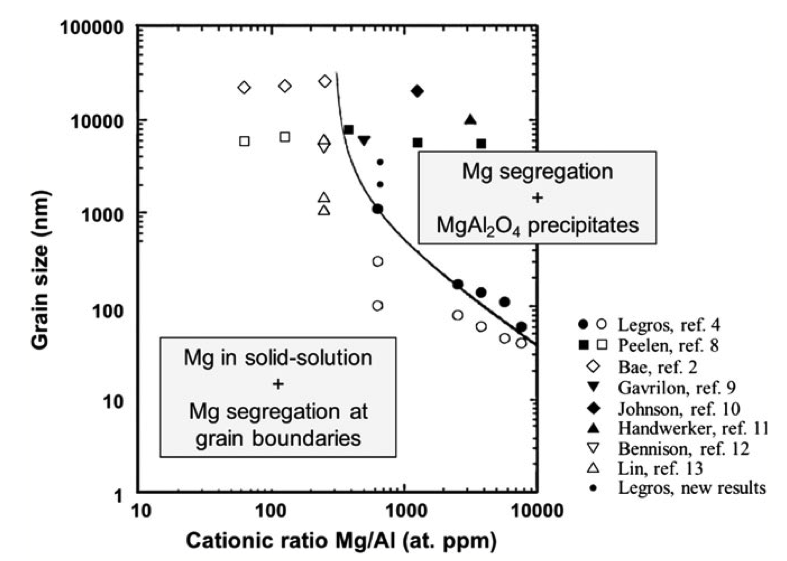
\includegraphics{Chapter-1/Figures/Figure1.png}
	\caption{SIMS maps of Al$_{2}$O$_{3}$ doped with 500 ppm MgO (a) and 1000 ppm SiO$_{2}$ (b). Samples were sintered for 8 h at 1650$^{\circ}$C \cite{Gavrilov1999}.}
	\label{Ch1-figure:Figure1}
\end{figure}
%%%

\newpage
%%%
\begin{figure}[H]
	\centering
	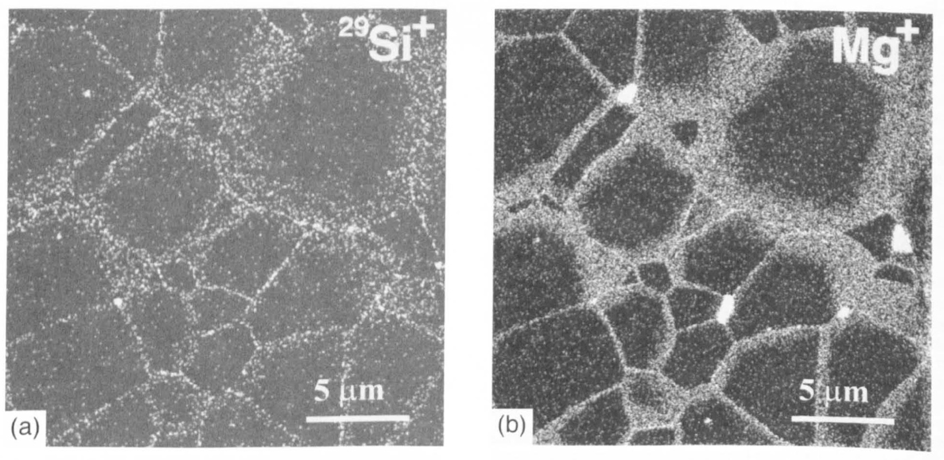
\includegraphics{Chapter-1/Figures/Figure2.png}
	\caption{SIMS maps of Al$_{2}$O$_{3}$ co-doped with 500 ppm MgO and 1000 ppm SiO$_{2}$ and sintered at 1650$^{\circ}$C for 8h. (a) shows the distribution of SiO$_{2}$, (b) the distribution of MgO in the same samples \cite{Gavrilov1999}.}
	\label{Ch1-figure:Figure2}
\end{figure}
%%%